% Guides
% http://ivk.knteu.kiev.ua/docum/z_vg.pdf
% http://www.ivk.knteu.kiev.ua/docum/prav01.pdf
\documentclass[a4paper,14pt,oneside,final]{extarticle}
\usepackage[top=2cm, bottom=2cm, left=3cm, right=1cm]{geometry}
\usepackage{scrextend}

\usepackage[T2A,T1]{fontenc}
\usepackage[ukrainian,russian,english]{babel}
\usepackage{tempora}
\usepackage{fontspec}
\setmainfont{tempora}

% Зачем: Отключает использование изменяемых межсловных пробелов.
% Почему: Так не принято делать в текстах на русском языке.
\frenchspacing

\usepackage{indentfirst}
\setlength{\parindent}{1.25cm}
\renewcommand{\baselinestretch}{1.5}

% Header
\usepackage{fancyhdr}
\pagestyle{fancy}
\fancyhead{}
\fancyfoot{}
\fancyhead[R]{\small \selectfont \thepage}
\renewcommand{\headrulewidth}{0pt}

% Captions
\usepackage{chngcntr}
\counterwithin{figure}{section}
\counterwithin{table}{section}
\usepackage[tableposition=top]{caption}
\usepackage{subcaption}
\DeclareCaptionLabelFormat{gostfigure}{Рисунок #2}
\DeclareCaptionLabelFormat{gosttable}{Таблиця #2}
\DeclareCaptionLabelSeparator{gost}{~---~}
\captionsetup{labelsep=gost}
\captionsetup[figure]{labelformat=gostfigure}
\captionsetup[table]{labelformat=gosttable}
\renewcommand{\thesubfigure}{\asbuk{subfigure}}

% Sections
\usepackage[explicit]{titlesec}
\newcommand{\sectionbreak}{\clearpage}

\titleformat{\section}
  {\centering}{\thesection \quad}{0pt}{\MakeUppercase{#1}}
\titleformat{\subsection}[block]
  {\bfseries}{\thesubsection \quad #1}{0cm}{}

\titlespacing{\section} {0cm}{0cm}{21pt}
\titlespacing{\subsection} {\parindent}{21pt}{0cm}
\titlespacing{\subsubsection} {\parindent}{0cm}{0cm}

% Lists
\usepackage{enumitem}
\renewcommand\labelitemi{--}
\setlist[itemize]{noitemsep, topsep=0pt, wide}
\setlist[enumerate]{noitemsep, topsep=0pt, wide, label=\arabic*}
\setlist[description]{labelsep=0pt, noitemsep, topsep=0pt, leftmargin=2\parindent, labelindent=\parindent, labelwidth=\parindent, font=\normalfont}

% Toc
\usepackage{tocloft}
\tocloftpagestyle{fancy}
\renewcommand{\cfttoctitlefont}{}
\setlength{\cftbeforesecskip}{0pt}
\renewcommand{\cftsecfont}{}
\renewcommand{\cftsecpagefont}{}
\renewcommand{\cftsecleader}{\cftdotfill{\cftdotsep}}

\usepackage{float}
\usepackage{pgfplots}
\usepackage{graphicx}
\usepackage{multirow}
\usepackage{amssymb,amsfonts,amsmath,amsthm}
\usepackage{csquotes}

\usepackage{listings}
\lstset{basicstyle=\footnotesize\ttfamily,breaklines=true}
\lstset{language=Matlab}

\usepackage[
	backend=biber,
	sorting=none,
	language=auto,
	autolang=other
]{biblatex}
\DeclareFieldFormat{labelnumberwidth}{#1}


\usepackage{lastpage}
\usepackage{calc}
\usepackage{soul}
\usepackage{pbox}
\usepackage{ulem}
\usepackage{titling}
\usepackage{framed}
\usepackage{tabu}
\usepackage{appendix}
\usepackage{packages/tikz-uml}
\usepackage[nomain,acronym,toc,nogroupskip,xindy={glsnumbers=false}]{glossaries}
\usepackage[figure,table]{totalcount}

\makeglossaries
\newglossarystyle{mylist}{%  
 % put the glossary in the itemize environment:  
 \renewenvironment{theglossary}%  
   {\begin{itemize}[label={}]}{\end{itemize}}%  
 % have nothing after \begin{theglossary}:  
 \renewcommand*{\glossaryheader}{}%  
 % have nothing between glossary groups:  
 \renewcommand*{\glsgroupheading}[1]{}%  
 \renewcommand*{\glsgroupskip}{}%  
 % set how each entry should appear:  
 \renewcommand*{\glossentry}[2]{%  
 \item % bullet point  
 \glstarget{##1}{\glossentryname{##1}}% the entry name  
 \space ---% the symbol in brackets  
 \space \glossentrydesc{##1}% the description  
 \space [##2]% the number list in square brackets  
 }%  
 % set how sub-entries appear:  
 \renewcommand*{\subglossentry}[3]{%  
   \glossentry{##2}{##3}}%  
 } 
\setglossarystyle{mylist}
 
\graphicspath{{figures/}}
\addbibresource{bibliography.bib}

\newacronym{am}{АМ}{агентне моделювання}
\newacronym{gis}{ГІС}{геоінформаційна система}
\newacronym{computer}{ЕОМ}{електронна обчислювальна машина}
\newacronym{mas}{МАС}{мультиагентна система}
\newacronym{pc}{ПЕОМ}{персональна електронна обчислювальна машина}
\newacronym{sw}{ПЗ}{програмне забезпечення}
\newacronym{smw}{СУОП}{система управління охороною праці}

%\newacronym{afapl}{AFAPL}{Agent Factory Agent Programming Language}
%\newacronym{api}{API}{Application Programming Interface}
%\newacronym{corba}{CORBA}{Common Object Request Broker Architecture}
%\newacronym{fipa}{FIPA}{Foundation for Intelligent Physical Agents}
%\newacronym{faq}{FAQ}{Frequently Asked Questions}
%\newacronym{lgpl}{LGPL}{GNU Lesser General Public License}
%\newacronym{gui}{GUI}{Graphical User Interface}
%\newacronym{jade}{JADE}{Java Agent Development Framework}
%\newacronym{jre}{JRE}{Java Runtime Environment}
%\newacronym{jvm}{JVM}{Java Virtual Machine}
%\newacronym{json}{JSON}{JavaScript Object Notation}
%\newacronym{uml}{UML}{Unified Modeling Language}

\newcommand{\khpistudentgroup}{КН-34г}
\newcommand{\khpistudentname}{Чепурний~А.~С.}

\newcommand{\khpidepartment}{Програмна інженерія та інформаційні технології управління}
\newcommand{\khpititlewhat}{
	Лабораторна робота №\labnumber \\
	з предмету <<Моделювання систем>>
}
\newcommand{\khpititlewho}{
	Виконав: \\
	\hspace*{\parindent} ст. групи \khpistudentgroup \\
	\hspace*{\parindent} \khpistudentname \\
	Перевірила: \\
	\hspace*{\parindent} ст. в. каф. ПІІТУ \\
	\hspace*{\parindent} Єршова~С.~І. \\
	\hspace*{\parindent} ас. каф. ПІІТУ \\
	\hspace*{\parindent} Литвинова~Ю.~С. \\
}


\begin{document}
\Ukrainian

\begin{titlepage}

\begin{center}
	МІНІСТЕРСТВО ОСВІТИ І НАУКИ УКРАЇНИ \\
	НАЦІОНАЛЬНИЙ ТЕХНІЧНИЙ УНІВЕРСИТЕТ \\
	«ХАРКІВСЬКИЙ ПОЛІТЕХНІЧНИЙ ІНСТИТУТ» \\[0.5cm]
	Кафедра <<\khpidepartment>> \\
\end{center}

\vspace{6cm}

\begin{center}
	\khpititlewhat
\end{center}

\vspace{3cm}

\begin{addmargin}[10cm]{0cm}
	\khpititlewho
\end{addmargin}

\vspace{\fill}

\begin{center}
	Харків \the\year
\end{center}

\end{titlepage}

\addtocounter{page}{7}
\renewcommand\contentsname{\hspace*{\fill}\bfseries\MakeUppercase{Зміст}\hspace*{\fill}}
\tableofcontents

\printglossary[type=\acronymtype,title={Перелік позначень та скорочень}]

\section*{Вступ}
\addcontentsline{toc}{section}{Вступ}

%Керуючись життєвим досвідом і науковими знаннями, людина будує моделі --- від паперових корабликів до картини світу. 
%Чим вони багатші і чим точніше ми можемо ними оперувати, тим краще наша свідомість --- наша <<найважливіша модель>>, відповідає реальності і знаходить способи її зміни.

% NaUKMAkn_2013_151_16.pdf
% http://www.economy.in.ua/pdf/1_2016/9.pdf
На сучасному етапі розвитку складні логістичні системи вимушені працювати в умовах високої невизначеності, що суттєво ускладнює управління ними. 
В процесі прийняття управлінських рішень виникає проблема прогнозування поведінки системи та зовнішнього середовища. 
Результати прогнозів необхідно постійно коригувати по ходу розвитку подій, що дозволяє пристосовуватися до змін оточення та гнучко реагувати на негативні впливи. 

У нагоді тут стає агентне моделювання, яке сягає своїм історичним корінням складних адаптивних систем і принципу побудови систем знизу вгору.
Агентне моделювання дозволяє здійснити множину прогнозів за різними сценаріями залежно від формування різноманітних ситуацій практично необмеженої складності. 

Основними елементами агентного моделювання є агенти, стосунки між ними і простір, в якому відбувається взаємодія. 
Агенти моделюються індивідуально. 
Вони можуть мати неповну інформацію, здійснювати помилки, адаптуватися до ситуації, проявляти ініціативу. 
В основу агентного моделювання закладені такі принципи, як різноманітність, взаємозв’язок і міра взаємодії. 
Тип взаємодій різних агентів може відрізнятися і носити ймовірнісний характер. 
Результатом динамічної взаємодії може бути певний рівноважний стан системи, а може бути і нова якість, яку неможливо передбачати з аналізу окремих складових системи.

Об'єктом дослідження є процес прийняття рішень розподільчою логістичною системою. 

Предметом дослідження є мультиагентна модель розподільчої логістичною системи. 

Теоретико-методологічною основою роботи є агентне моделювання, системний аналіз, а також базова теорія логістики.

Метою і завданням дослідження є розробка мультиагентної системи для дослідження розподільчої логістичної системи.
Для досягнення поставленої мети в курсовій роботі були сформульовані та вирішені наступні задачі:
\begin{itemize}
	% logistics
	\item описати динаміку розподільчої логістичної системи;
	\item дослідити проблеми імітаційного моделювання розподільчої логістичної системи;
	% agents
	\item порівняти фреймворки для реалізації мультиагентних систем, обрати та обґрунтувати вибір фреймворку;
	\item розробити специфікацію мультиагентної системи;
	\item реалізувати мультиагентну систему;
	\item верифікувати розроблену мультиагентну систему;
	\item протестувати мультиагентну систему на реальних даних;
	\item викласти пропозиції щодо перспектив розвитку та удосконалення розробленої мультиагентної системи.
\end{itemize}

%\section{Аналіз існуючих моделей і алгоритмів управління логістичними системами. Постановка задачі}
\section{Аналіз предметної області}
\subsection{Розподільча логістична система як об'єкт дослідження}
% https://essuir.sumdu.edu.ua/bitstream/123456789/38038/1/Bilovodska_Kyslyi_Olefirenko_Solyanyk.pdf
Розподільча логістика --- це частина загальної логістичної системи, яка забезпечує найбільш ефективну організацію розподілу продукції, охоплюючи систему товароруху і виконуючи логістичні операції транспортування, складування, упакування та ін.~\cite{Kusluy2010}.

Розподільча логістика спрямована на комплексне планування, управління та фізичне опрацювання потоку готових виробів у супроводі необхідного інформаційного, фінансового та сервісного потоку від моменту здачі-приймання товарів з виробництва до замовника (споживача) з метою оптимізації витратних та часових характеристик зазначеної частини матеріального і нематеріального потоків.
Головна мета розподільчої логістики --- організація розподільчої діяльності відповідно до замовлень клієнтів з мінімальними загальними витратами~\cite{Kusluy2010}.

Принципова відмінність розподільчої логістики від традиційного розуміння збуту полягає насамперед у системному взаємозв'язку процесу розподілу з процесами виробництва і закупівель під час управління матеріальними потоками, а також системному взаємозв'язку всіх функцій всередині самого розподілу.

Матеріальний потік у сфері розподілу має форму готової продукції.
Залежно від суб'єкту економічних відносин, який бере участь у доведенні ресурсів до споживача, потік готової продукції можна подати як товарний потік або як вантажний потік (на транспорті).

Розподільча логістика будується на загальних логістичних принципах~\cite{Anikin1999}:
\begin{itemize}
	\item координація всіх процесів товароруху, починаючи від кінцевих операцій товаровиробника та закінчуючи сервісом споживача;
	\item інтеграція всіх функцій управління процесами розподілу готової продукції та послуг, починаючи від визначення мети та закінчуючи контролем;
	\item адаптація комерційного, канального та фізичного розподілу до постійно змінних вимог ринку та потреб споживача;
	\item координація всіх процесів товароруху, починаючи від кінцевих операцій товаровиробника та закінчуючи сервісом споживача;
	\item системність як управління розподілом в його цілісності та взаємозалежності всіх елементів збутової діяльності;
	\item комплексність, тобто вирішення всієї сукупності проблем, пов’язаних із задоволенням платоспроможного попиту покупців;
	\item оптимальність стосовно як елементів системи, так і режиму її функціонування;
	\item раціональність як в організаційній структурі, так і в організації управління.
\end{itemize}

Склад завдань розподільчої логістики на мікро- та на макрорівні різний~(таблиця~\ref{tab:logistic_functions}). 

\begin{table}[H]
	\caption{Завдання розподільчої логістики на мікро- та макрорівнях}
	\label{tab:logistic_functions}
	\begin{tabular}{@{}|p{0.53\linewidth}|p{0.4\linewidth}|@{}}
	 	\hline
		Мікрорівень & Макрорівень \\ \hline
		\begin{itemize}[leftmargin=*]
			\item оптимізація формування портфеля замовлень;
			\item укладання договорів із замовниками на постачання продукції;
			\item забезпечення ритмічності та дотримання планомірності реалізації продукції;
			\item вивчення і задоволення потреб у логістичному сервісі;
			\item раціоналізація параметрів, структури і просування динамічних матеріальних потоків;
			\item оптимізація параметрів і умов зберігання запасів товарного характеру;
			\item формування і вдосконалення системи інформаційного забезпечення.
		\end{itemize}
		&
		\begin{itemize}[leftmargin=*]
			\item вибір схеми розподілу матеріального потоку;
			\item визначення оптимальної кількості розподільчих центрів на території, яка обслуговується;
			\item визначення оптимального місця розташування розподільчого центру на території, яка обслуговується, та ін.
		\end{itemize} \\ \hline
	\end{tabular}
\end{table}

\subsection{Проблеми моделювання і управління розподільчими логістичними системами}
Основною проблемою, характерною для об'єкта дослідження, яка породжує безліч інших проблем, є його ієрархічність і розподіленість. 
В таких системах процеси розосереджені по окремих підсистемах і знаходяться на різних рівнях ієрархії. 
Для таких систем вирішується комплекс взаємопов'язаних задач в режимі багатосторонньої взаємодії між менеджерами-аналітиками, що відповідають за окремі локальні завдання і \acrshort{computer}. 
Основними ознаками розподіленості будь-якої логістичної системи можна вважати:
\begin{itemize}
	\item наявність механізму розбиття даної системи на окремі взаємопов'язані підсистеми;
	\item окремі складові системи географічно відокремлені;
	\item відносна автономність окремих підсистем;
	\item спільне завдання всієї системи розглядається у вигляді набору окремих локальних підзадач;
	\item паралельність і асинхронність рішення окремих локальних задач різними виконавцями.
\end{itemize}

Першою проблемою, яку необхідно вирішувати, є розбиття кожної системи на окремі локальні підсистеми. 
Можна сказати, що формалізація цих двох завдань здійснюється на основі декомпозиції і агрегування. 
Декомпозиція полягає в розчленуванні вихідної задачі на ряд відносно незалежних підзадач, а агрегування --- в заміні окремих груп змінних, що характеризують ефективність функціонування системи, змінними-агрегатами. 
При цьому висувається вимога повної (достатньої) еквівалентності задач. 
Агрегування параметрів і змінних здійснюється в ході руху вгору по ієрархії. 
Це пов'язано з великою розмірністю завдання і неможливістю прийняття рішень на основі варіювання всіх параметрів і змінних. 
Основні ідеї, які реалізуються при синтезі моделі на основі декомпозиції і агрегування полягають у наступному:
\begin{itemize}
\item нехтуючи слабкими зв'язками між окремими підсистемами, зробити декомпозицію;
\item використовуючи трохи відмінності між ними, зробити агрегування;
\item використовуючи сильні відмінності, виділити <<вузькі місця>>, відкинувши на основі апріорних оцінок несуттєві обмеження.
\end{itemize}

\subsection{Моделі логістичних систем}
Моделювання в загальному вигляді являє собою один з основних методів пізнання, є формою відображення дійсності і полягає у з'ясуванні або відтворенні тих чи інших властивостей реальних об'єктів, процесів, явищ за допомогою абстрактного опису у вигляді зображення, плану, карти, сукупності рівнянь, алгоритмі і програм.

Одним з найбільш ефективних методів дослідження складних систем розподільчої логістики є імітаційне моделювання~\cite{Kobelev2003}.

Імітаційне моделювання --- експериментальний метод дослідження реальної системи за її імітаційною моделлю, який поєднує особливості експериментального підходу і специфічні умови використання обчислювальної техніки~\cite{Emelyanov2002}.

Серед переваг імітаційного моделювання відзначають~\cite{Emelyanov2002}: 
\begin{enumerate}
	\item Відображення динамічних процесів і поведінкових аспектів зовнішнього середовища.
	\item Можливість виявлення закономірностей, динамічних тенденцій розвитку і функціонування складної системи в умовах неповної та неточної інформації.
	\item Опис взаємодії та поведінки безлічі активних агентів в соціальних системах.
	\item Реалізацію принципів об'єктно-орієнтованого проектування і застосування високотехнологічних рішень при побудові комп'ютерних моделей та ін.
\end{enumerate}

Головною проблемою при побудові будь імітаційної моделі є необхідність побудови комплексних математичних моделей і розробки програмного коду імітаційної моделі. 

У імітаційному моделюванні виділяють такі основні підходи:
\begin{itemize}
	\item системна динаміка;
	\item дискретне моделювання;
	\item агентне моделювання.
\end{itemize}

\subsubsection{Системна динаміка}
Як методологія системна динаміка була запропонована в 1961 році Дж. Форрестером в якості інструменту дослідження інформаційних зворотних зв'язків у виробничо-господарської діяльності. 
Процеси, що відбуваються в реальному світі, в системній динаміці представляються в термінах накопичувачів і потоків між ними.
Системнодинамічна модель описує поведінку системи та її структуру як безліч взаємодіючих зворотних зв'язків і затримок. 
Математично така модель виглядає як система диференціальних рівнянь. 
Результатом моделювання в системній динаміці є виявлення глобальних залежностей і причинно-наслідкових зв'язків у досліджуваній системі~\cite{Shamrin2016}. 

\subsubsection{Дискретне моделювання}
Основний об'єкт в системі дискретного моделювання --- пасивний транзакт, який може певним чином представляти собою працівників, деталі, сировину, документи, сигнали і т. п.
Переміщаючись по моделі, транзакти стають в черги до одноканальним і багатоканальним пристроям, захоплюють і звільняють їх, розщеплюються, знищуються і т. д.
Відмінною особливістю даного підходу є час просування по моделі: або від події до події, або через дискретні проміжки часу. 
Дискретне моделювання застосовується, якщо можливо припустити, що змінні в системі змінюються миттєво в певні проміжки часу. 
Даний підхід імітаційного моделювання є одним з найпоширеніших і застосовується для дослідження соціально-економічних, технічних, логістичних та інших процесів.
На основі дискретного підходу реалізовано найбільше
число систем імітаційного моделювання~\cite{Shamrin2016}. 

\subsubsection{Агентне моделювання}
Агентське моделювання з'явилося в 90-х роках і використовується для дослідження децентралізованих систем, динаміка функціонування яких визначається не глобальними правилами і законами (як в інших парадигмах моделювання), а коли ці глобальні правила і закони є результатом індивідуальної активності членів групи.

Агентно-орієнтована система може складатися з одного агента (наприклад, програмний секретар~\cite{Maes1995}), проте весь потенціал розкривається з використанням мультиагентної системи~\cite{Waters1989}.
Під агентом розуміється система, яка має такі властивості~\cite{Jennings1998,Wooldridge1995}:
\begin{enumerate}[label={\arabic*)}]
	\item автономність: агенти мають внутрішній стан (який недоступний іншим агентам) та приймають рішення на основі своїх даних, без прямого втручання людини;
	\item реактивність: агенти розміщуються в навколишньому середовищі (яке може бути фізичним світом, множиною інших агентів, інтернетом і т.д.), здатні спостерігати і своєчасно реагувати на зміни;
	\item проактивність: агенти не тільки реагують на зміни в зовнішньому середовищі, вони здатні виявляти ініціативу для досягнення своєї мети;
	\item соціальність: агенти взаємодіють з іншими агентами (і, можливо, людиною) через спеціальний інтерфейс для досягнення їх цілей.
\end{enumerate}

Мета агентських моделей --- отримати уявлення про ці глобальні правила, загальну поведінку системи, виходячи з припущень про індивідуальну, приватну поведінку її окремих активних об'єктів і взаємодію цих об'єктів в системі.
У разі моделювання логістичних систем, що містять великі кількості активних об'єктів (людей, машин, підприємств чи навіть проектів, активів, товарів і т. п.), які об'єднує наявність елементів індивідуальної поведінки, агентське моделювання є підходом більш універсальним і потужним, оскільки дозволяє врахувати будь-які складні структури та їх поведінку~\cite{Shamrin2016}. 

\subsection{Глосарій проекту}
Глосарій проекту --- це розвернутий словник у вигляді таблиці, який складається з термінів що характеризують дану предметну область.

Глосарій проекту:
\begin{enumerate}
    \item Агент \textit{(agent)} --- це сутність, що спостерігає за навколишнім середовищем і діє у ньому, при цьому його поведінка раціональна в тому розумінні, що він здатен до розуміння і його дії завжди спрямовані на досягнення якої-небудь мети~\cite{Jennings1998}.
    \item Транспорт \textit{(transport)} --- сукупність засобів, для переміщення людей, вантажів, сигналів та інформації з одного місця в інше.
    \item Склад \textit{(warehouse)} --- це складна технічна споруда, яка складається із взаємопов'язаних елементів, що має певну структуру та виконує ряд функцій з перетворення матеріальних потоків, а також накопичення, переробки та розподілу вантажів між споживачами~\cite{Kusluy2010}. 
	\item Запаси гарантійні \textit{(insurance stocks)} призначені для безперервного постачання споживачів у випадку непередбачених обставин: відхилення в періодичності та величині партій поставок від запланованих, зміни інтенсивності споживання, затримки поставок та ін. і є постійною величиною, що залежить від умов виконання конкретних поставок~\cite{Kusluy2010}. 
	\item Ланцюг логістичний \textit{(logistics chain)}  --- це складна система, що формується впорядкованою і взаємодіючою сукупністю фізичних чи юридичних осіб на ринку виробництва і постачання матеріальних ресурсів, виробництва та розподілу продукції, які виконують логістичні операції, спрямовані на доведення матеріального потоку від однієї логістичної системи до іншої та до кінцевого споживача~\cite{Kusluy2010}.  
    \item Логістика \textit{(logistics)} --- системоохоплюючий механізм, який можна трактувати як досягнення компромісу (узгодження) між виконанням зобов’язань і необхідними для цього витратами в сфері виробництва, транспортно-складського забезпечення, у процесі отримання потрібних товарів або послуг у потрібному місці, у потрібний час, у необхідній кількості з мінімальними загальними витратами при високій якості обслуговування споживача~\cite{Kusluy2010}.
	\item Логістика розподільча \textit{(distribution logistics)} --- галузь логістики, яка забезпечує найбільш ефективну організацію розподілу продукції, охоплюючи систему товароруху і виконуючи логістичні операції транспортування, складування, упакування та ін.~\cite{Kusluy2010}.
	\item Рівень сервісу \textit{(service level)} --- кількісна характеристика відповідності фактичних значень показників якості і кількості логістичних послуг оптимальним або теоретично можливим значенням~\cite{Kusluy2010}.
    \item Операції логістичні \textit{(logistic operations)} --- відособлена сукупність дій, скерована на перетворення матеріального та супутніх йому потоків~\cite{Kusluy2010}.
    \item Сервіс логістичний \textit{(logistic service)} --- це сукупність функцій і видів діяльності всіх підсистем підприємства, що забезпечують зв’язок <<підприємство-споживач>> для кожного матеріального та інформаційного потоку за показниками номенклатури, якості, кількості, ціни, місця і часу постачання продукції відповідно до вимог ринку~\cite{Kusluy2010}.
\end{enumerate}

\subsection{Постановка задачі}
Завданням дипломної роботи є розробка мультиагентної системи для дослідження різних конфігурацій розподільчої логістичної системи.

Розроблена система повинна мати простий графічний інтерфейс та бути зручною для використання. 

Даний програмний продукт може бути використаний логістичними компаніями з метою покращення сервісу, викладачами та студентами для дослідження логістичних систем.

Для розробки даної системи необхідно вирішити наступні задачі:
\begin{itemize}
	% logistics
	\item опис динаміки розподільчої логістичної системи;
	\item дослідження проблеми імітаціонного моделювання розподільчої логістичної системи, опис різних моделей;
	% agents
	\item порівняння фреймворкій для реалізації мультиагентних систем, обрання та обґрунтування вибору;
	\item розробка специфікації мультиагентної системи;
	\item реалізація мультиагентної системи;
	\item тестування мультиагентної систему;
	\item викладення пропозиції щодо перспектив розвитку та удосконалення розробленої мультиагентної системи.
\end{itemize}

\section{Проектування системи відстеження напрямку погляду}
\subsection{Розробка вимог до програмної системи}
\subsubsection{Галузь застосування}
Данний продукт може бути використаний медичними програмами (контролювання курсору миші поглядом), та в цілях сбору пасивної інформації про точку погляду користувача персонального комп'ютера.

\subsubsection{Функціональні вимоги}
Список функціональних вимог до системи:
\begin{enumerate}[label={\arabic*)}]
	\item система повинна мати можливість налаштування під навколишнє середовище (тип веб-камери, положення мониторів комп'ютера);
	\item система повинна визначати точку погляду користувача з похобкою не більше ніж 5 см.;
	\item система повинна працівати з однією веб-камерою.  
\end{enumerate}

\subsubsection{Нефункціональні вимоги}
Список нефункціональних вимог до системи:
\begin{enumerate}[label={\arabic*)}]
	\item система повинна бути платформонезалежною та підтримувати такі операційні системи, як Debian, Windows, macOS;
	\item система повинна бути не вимогливою до веб-камери та комп'ютеру;
\end{enumerate}

\subsection{Архітектура програмної системи}
Для реалізації системи була обрана однорівнева архітектура \textit{(standalone application)}.

Однорівнева архітектура була обрана через те, що для відстеження напрямку погляду необхідно обробляти відеопоток, що потребуватиме надсилання великого об'єму данних на сервер.
Цей спосіб буде потребувати багато ресурсів сервера та може стати проблемою для конфіденціальності користувача.  

\subsubsection{Діаграма компонентів}
На рисунку~\ref{fig:component} зображена діаграма компонентів системи.

\begin{figure}[H]
	\centering
	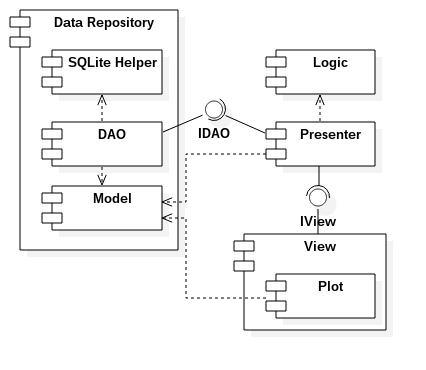
\includegraphics{uml_component}
	\caption{UML-діаграма компонентів}
	\label{fig:component}
\end{figure} 

Головними компонентами є:
\begin{itemize}
	\item \texttt{opencv} --- бібліотека функцій та алгоритмів комп'ютерного зору, обробки зображень і чисельних алгоритмів загального призначення з відкритим кодом;
	\item \texttt{keras} --- відкрита нейромережева бібліотека, написана мовою Python;
	\item \texttt{tensorflow} --- відкрита програмна бібліотека для машинного навчання цілій низці задач, розроблена компанією Google;
	\item \texttt{dlib} --- відкрита програмна бібліотека для машинного навчання;
	\item \texttt{gradients} --- реалізація методу середніх градієнтів;
	\item \texttt{main} --- головна компонента програми .
\end{itemize}

\subsubsection{Діаграма послідовності}
На рисунку~\ref{fig:sequence} зображена діаграма послідовності системи.

\begin{figure}[H]
	\centering
	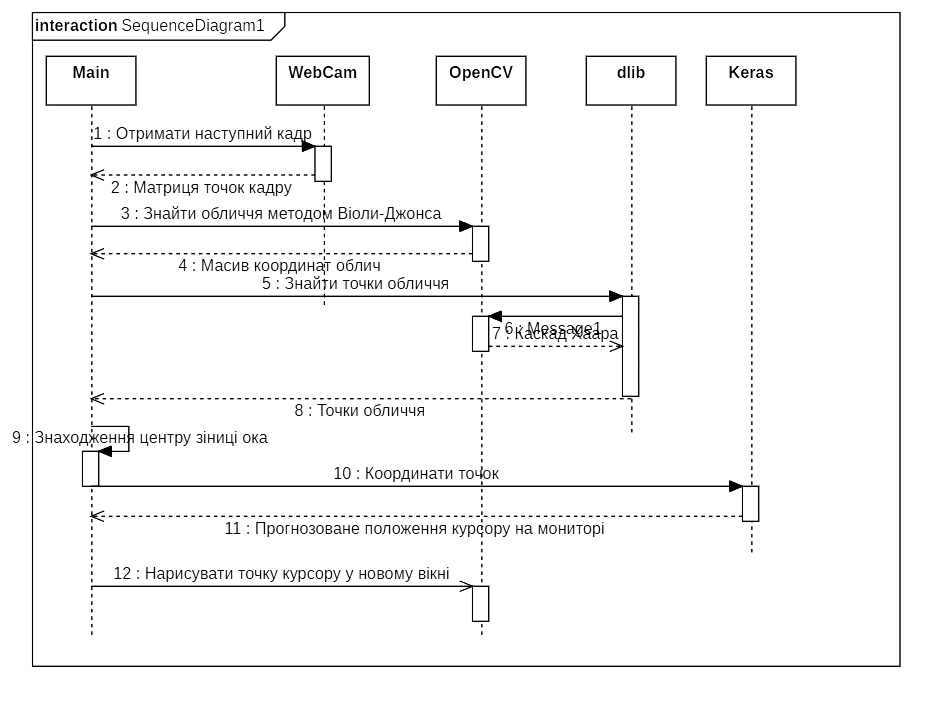
\includegraphics[width=\textwidth]{uml_sequence}
	\caption{UML-діаграма послідовності}
	\label{fig:sequence}
\end{figure} 

\subsubsection{Схема нейронної мережі}
На рисунку~\ref{fig:network} зображена схема нейронної мережі.

\begin{figure}[H]
	\centering
	\includegraphics[width=\textwidth]{network}
	\caption{Схема нейронної мережі}
	\label{fig:network}
\end{figure} 

Нейронна мережа буде складатися з п'яти шарів:
\begin{enumerate}[label={\arabic*-й ---}]
	\item має форму $256\times2$ та лінійну функцію активації; 
	\item має форму $128\times2$ та лінійну функцію активації; 
	\item має форму $64\times2$ та лінійну функцію активації; 
	\item має форму $256\times1$ та функцію активації сігмоїда; 
	\item має форму $2\times1$ та функцію активації сігмоїда. 
\end{enumerate}

На вхід подається матриця нормалізованих координат специфічних точок обличчя, які зображені на рисунку~\ref{fig:face}. 

\begin{figure}[H]
	\centering
	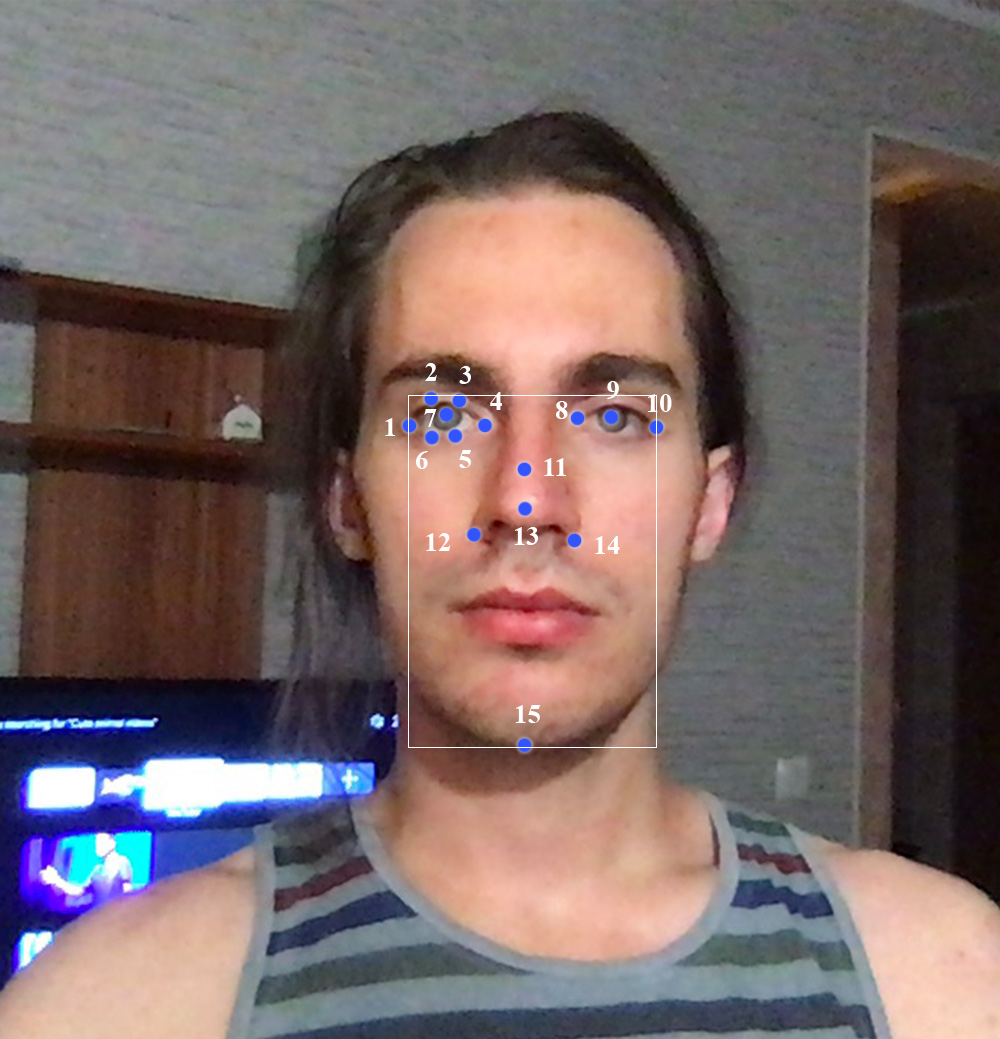
\includegraphics[width=0.6\textwidth]{face}
	\caption{Точки, які використовуються для визначення погляду}
	\label{fig:face}
\end{figure} 

\subsection{Обґрунтування вибору платформи розробки та інструментальних засобів}
\subsubsection{Мова програмування Python}
Python чудово підходить для вирішення задач машинного навчання, дозволяя писати стислий та експресивний код.

\subsubsection{Система управління версіями Git}
Використання системи контролю версії є необхідним для роботи над великими проектами.

Система контролю дозволяє зберігати попередні версії файлів та завантажувати їх за потребою. 
Вона зберігає повну інформацію про версію кожного з файлів, а також повну структуру проекту на всіх стадіях розробки.

Git --- розподілена система керування версіями файлів та спільної роботи. Git є однією з найефективніших, надійних і високопродуктивних систем керування версіями, що надає гнучкі засоби нелінійної розробки, що базуються на відгалуженні і злитті гілок.

\subsubsection{Середовище розробки застосунків Sublime Text 3}
Sublime Text 3 --- швидкий кросплатформенний редактор вихідних текстів програм. Підтримує плагіни, розроблені за допомогою мови програмування Python.

\section{Результати застосування розробленої системи}
\subsection{Стислі відомості щодо розгортання системи}

Вимоги до серверної машини наведено у таблиці~\ref{tab:sw_requirements}. 

\begin{table}[h]
	\caption{Мінімальні вимоги до серверного обладнання}
	\label{tab:sw_requirements}
	\begin{tabular}{l|l}
		Процесор & 1000 МГц \\ \hline
		ОЗП & 512 МБ \\ \hline
		Об'єм пам'яті диску & 64 ГБ 
	\end{tabular}
\end{table}

Програмне забезпечення серверу може бути встановлено на операційні системи родини \textit{Linux}, \textit{Windows} або \textit{macOS}.
Рекомендовано використовувати \acrshort{ssd} у якості накопичувача.

Для розгортання системи необхідно встановити наступні програми:
\begin{itemize}
	\item Apache Server v2.4.29+;
	\item SQLite v3.22.0+;
	\item PHP v7.2.2+;
\end{itemize}
та встановити драйвер взаємодії PHP з SQLite.

\subsection{Опис роботи з сайтом}
Робота з сайтом починається з процесу реєстрації користувача~(рисунок~\ref{fig:site_register}).
Незареєстрований користувач може переглядати товари та додавати їх до кошику, але не може оформити замовлення. 
\begin{figure}[H]
    \centering
    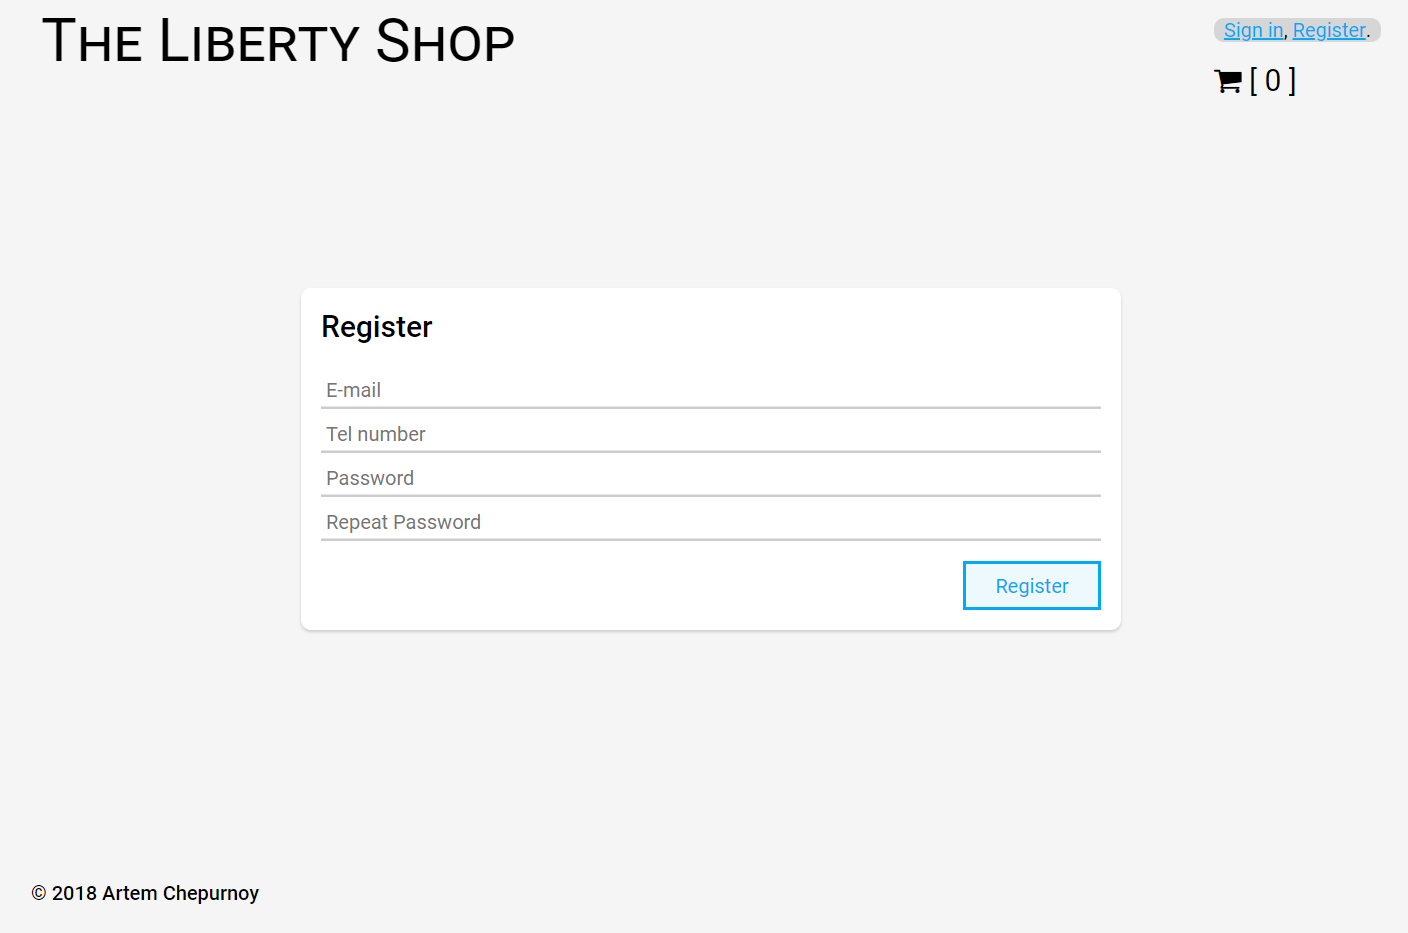
\includegraphics[width=0.8\textwidth]{screen_register}
    \caption{Сторінка реєстрації у системі}
    \label{fig:site_register}
\end{figure}

Після реєстрації користувач має увійти до системи~(рисунок~\ref{fig:site_login}).
\begin{figure}[H]
    \centering
    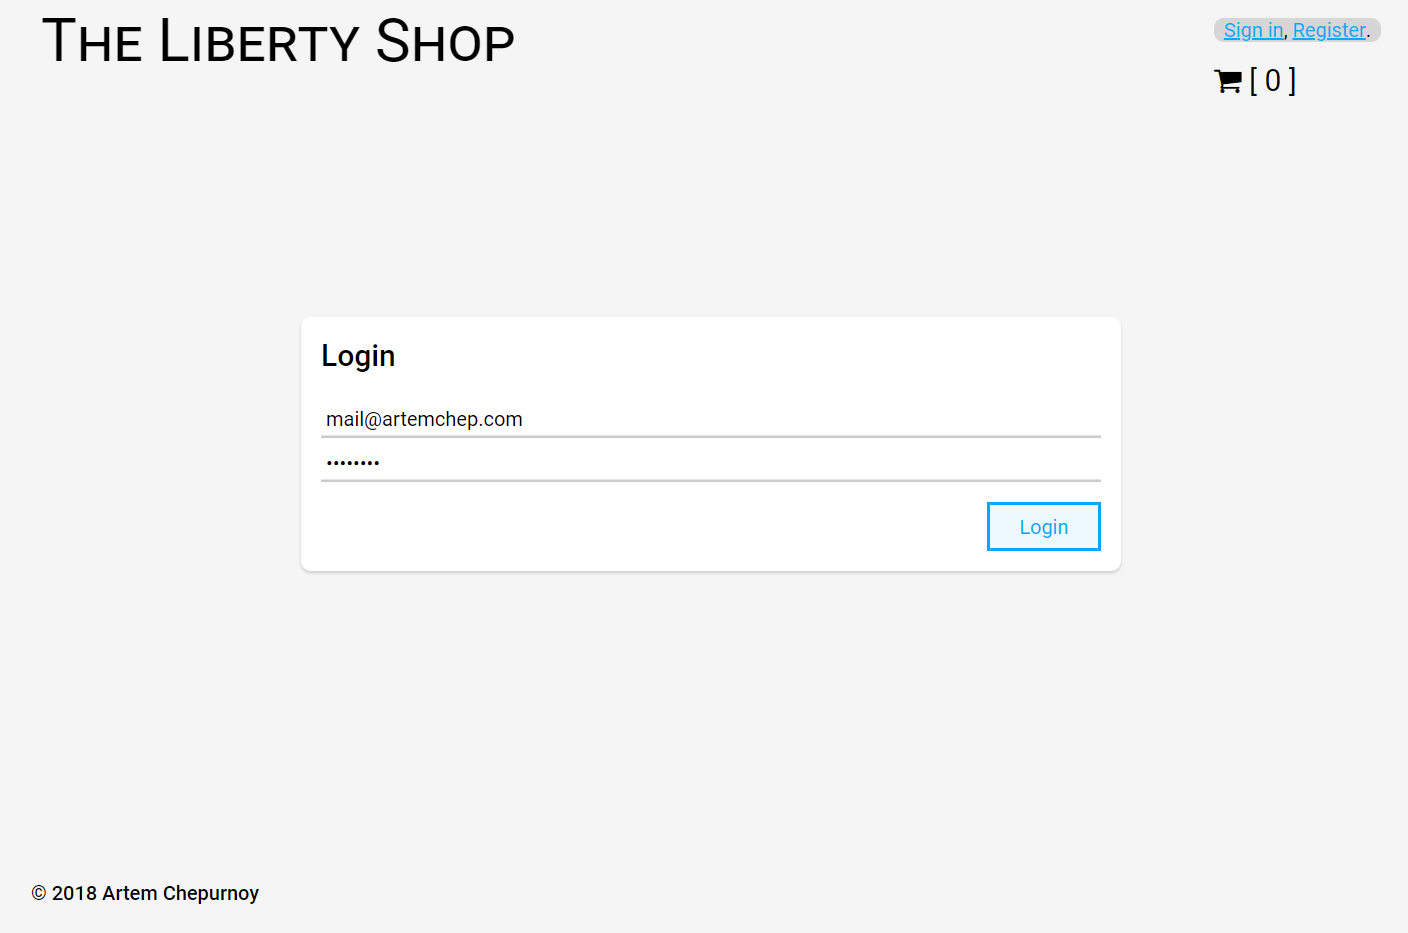
\includegraphics[width=0.8\textwidth]{screen_login}
    \caption{Сторінка входу до системи}
    \label{fig:site_login}
\end{figure}

Користувач може переглядати доступні товари на головній сторінці сайту.
Доступна можливість пошуку товару за ім'ям та категоріям.
\begin{figure}[H]
    \centering
    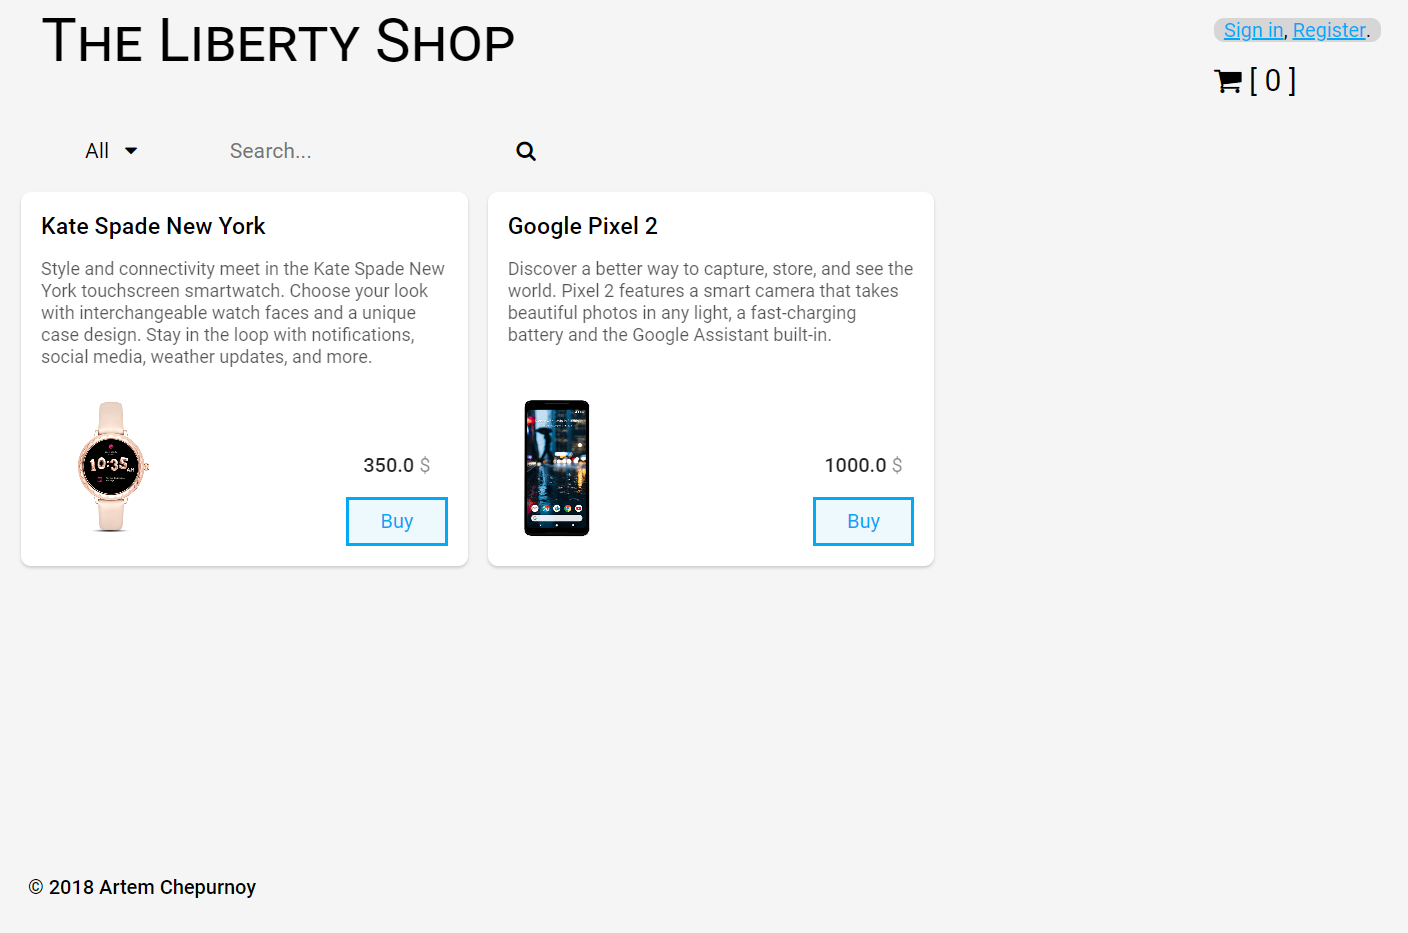
\includegraphics[width=0.8\textwidth]{screen_product__list}
    \caption{Головна сторінка ресурсу}
    \label{fig:site_product_list}
\end{figure}

Адміністратор та менеджери сайту мають на головній сторінці додаткові елементи~(рисунок~\ref{fig:site_product_list_admin}): 
\begin{itemize}
\item Кнопка редагування продуктів;
\item \textit{<<Add product>>} --- показати діалог додавання нового продукту;
\item \textit{<<Add category>>} --- показати діалог додавання нової категорії продуктів;
\item \textit{<<Edit category>>} --- показати діалог редагування та видалення категорії продуктів.
\end{itemize}
\begin{figure}[H]
    \centering
    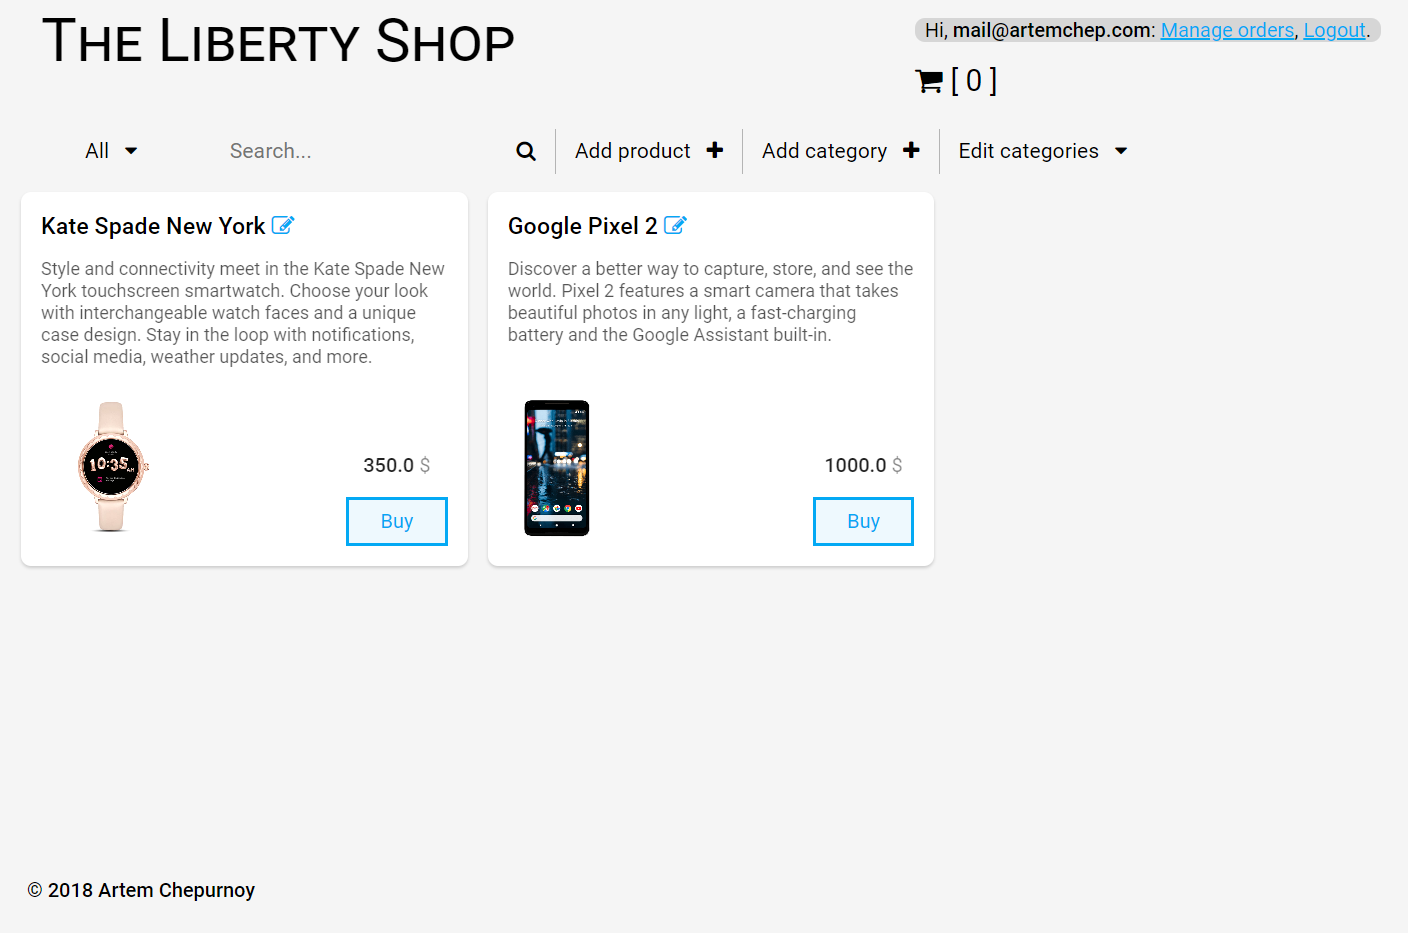
\includegraphics[width=0.8\textwidth]{screen_product__list__admin}
    \caption{Головна сторінка ресурсу (адміністратор)}
    \label{fig:site_product_list_admin}
\end{figure}

Діалог для створення нового продукту представлено на рисунку~\ref{fig:site_product_add}).

Продукт має такі властивості як категорія продуктів, назва, короткий опис, графічне зображення, ціна та розмірність.   
\begin{figure}[H]
    \centering
    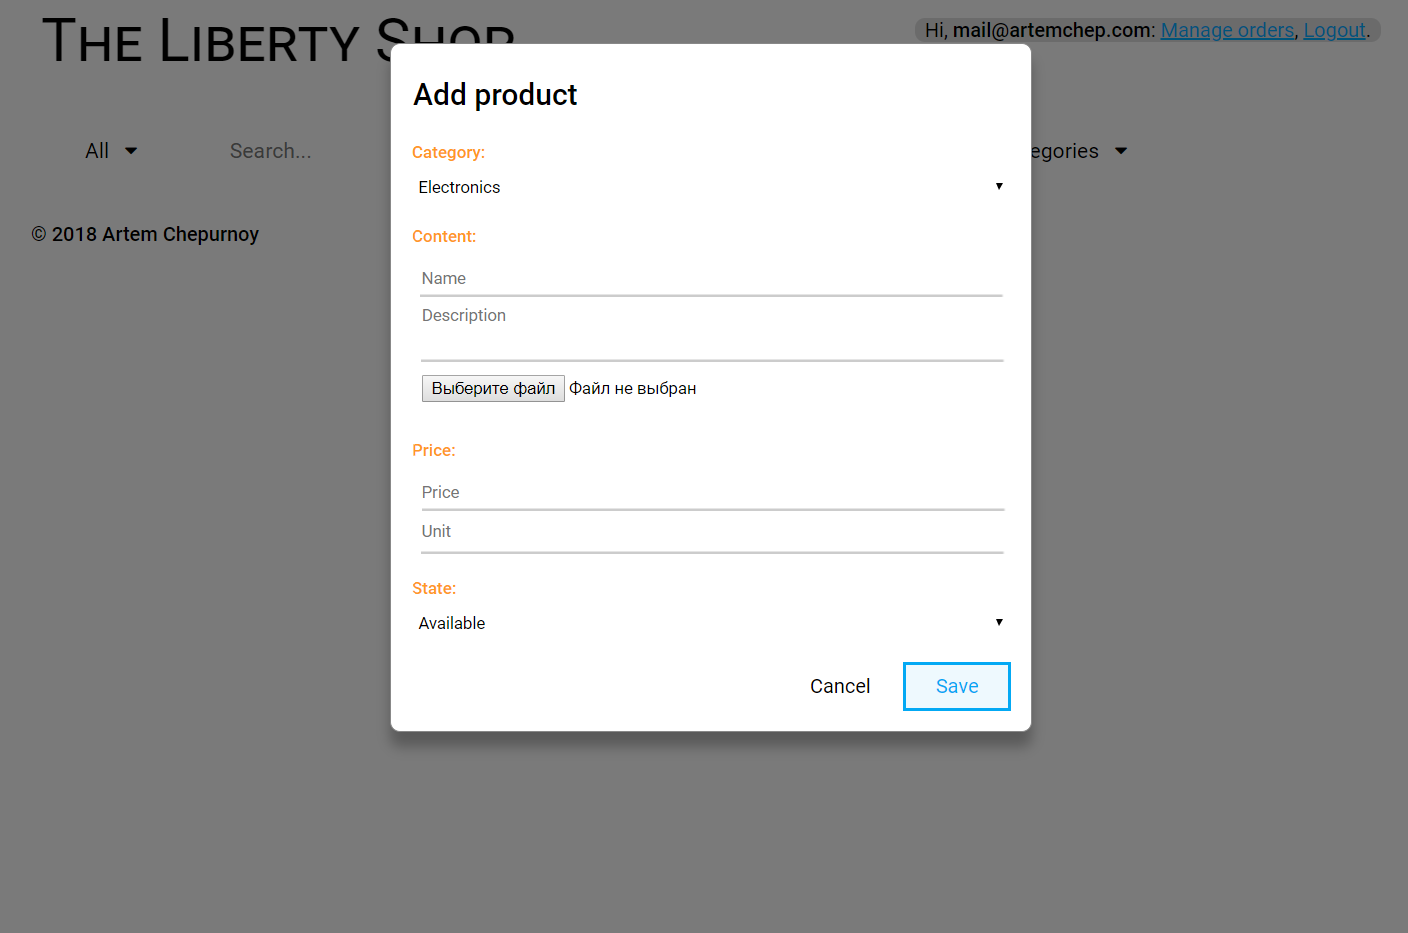
\includegraphics[width=0.8\textwidth]{screen_product_add}
    \caption{Діалог створення нового продукту}
    \label{fig:site_product_add}
\end{figure}

Адміністратор та менеджер ресурсу мають можливість переглянути список поточних або минулих замовлень~(рисунок~\ref{fig:site_order_list}), перемістити замовлення до архіву.
Є можливість фільтрування замовлень по даті створення, даті архівування, назві, категорії, кількості продуктів та ціні.   
\begin{figure}[H]
    \centering
    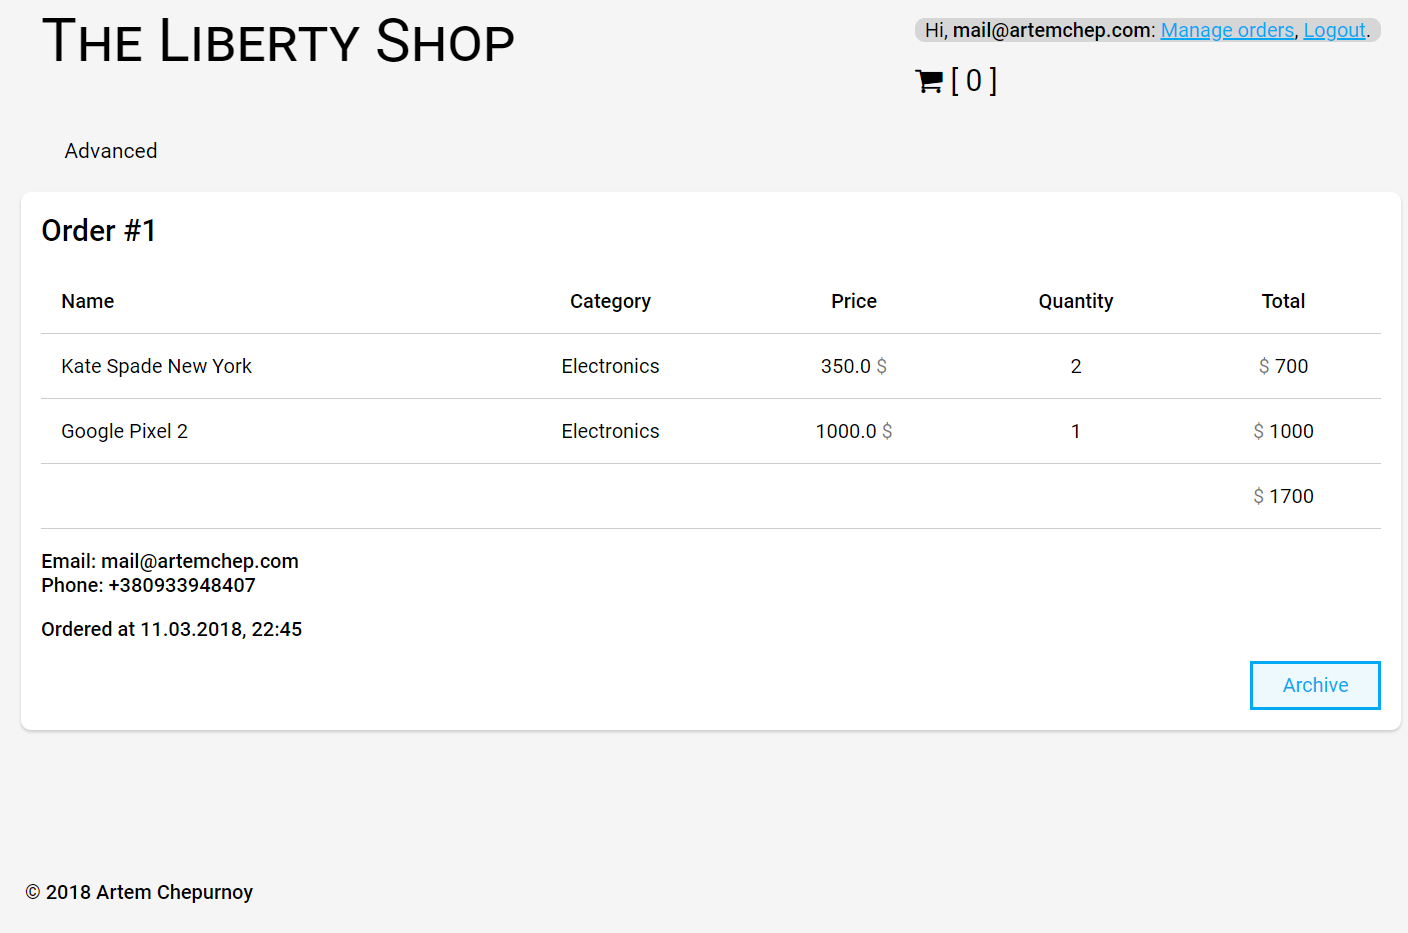
\includegraphics[width=0.8\textwidth]{screen_order__list}
    \caption{Сторінка керування замовленнями}
    \label{fig:site_order_list}
\end{figure}

\subsection{Результати тестування та рекомендації щодо удосконалення розробленої системи}
При тестуванні основною проблемою виявилася підтримка сайтом різних пристроїв та браузерів. 
При більш детальному вивченні стандартів HTML та CSS ця проблема була вирішена.

Одним із напрямків розвитку розробленої системи є співробітництво з іншими постачальниками, створення платформи для постачальників. 

\section*{Висновки}
\addcontentsline{toc}{section}{Висновки}
Сучасні алгоритми <<комп'юторного зору>> дозволяють досить швидко створювати вражаючі програми які реалізують зоровий інтерфейс.
Використання нейронних мереж спрощує задачу переведення точок обличчя у положення погляду не екрані.

В ході написання роботи дану задачу було розкрито повною мірою на прикладі проектування та реалізації програмної системи для визначення погляду користувача з видеоряду та керування курсором за допомогою погляду. 

В процесі дослідження були сформульовані вимоги до програмної системи, та обрана й спроектована її архітектура.
Обгрунтований вибір інструментальних засобів розробки.

\printbibliography[heading=bibintoc, title={Список джерел інформації}]


\begin{appendices}
	% custom commands 
	\newcommand\appendixsection[1]{
		\addtocounter{section}{1}
		\clearpage
		\section*{Додаток \thesection. #1}
		\addcontentsline{toc}{section}{Додаток \thesection. #1}
	}

	\appendixsection{Порівняння платформ для розробки мультагентних систем}
{
	\small
	\tabulinesep=1.2mm
	\begin{longtabu} to \textwidth {|X[2,l]|X[2,l]|X[3,l]|X[3,l]|}
  		\caption{Порівняння платформ для розробки \acrshort{mas}~\cite{Kravari2015}}
  		\label{tab:mas_platform_comparsion} \\
		\hline
		& \textbf{Agent Factory} & \textbf{\acrshort{jade}} & \textbf{AnyLogic} \\\hline\endfirsthead
  		\caption*{Продовження таблиці \thetable{}}\\
		\hline
		& \textbf{Agent Factory} & \textbf{\acrshort{jade}} & \textbf{AnyLogic} \\\hline\endhead
		% Platform properties
		Организація & University College Dublin & Telecom Italia (TILAB) & Компанія AnyLogic \\\hline
		Основна доменна область & Агенти для загального призначення & Розподілені мультиагентні системи & Розподілені мільтиагентні симуляції \\\hline
		Ліцензія & LGPL & LGPL & Комерційна та академічна ліцензії \\
		\hline
		% Usability overview
		Простота використання & Простий / Нестача функціоналу у \acrshort{gui} & Зручний, простий \acrshort{gui}, багато звичних функцій & Середній / Багатий функціонал \acrshort{gui} \\\hline
		Легкість вивчення платформи & Середня & Легка (багато прикладів) & Легка \\\hline
		Масштабованість & Добра & Висока & Висока \\\hline
		Сумісність зі стандартами & \acrshort{fipa} & \acrshort{fipa}, \acrshort{corba} & \acrshort{gis}, 3D-можливості \\
		\hline
		% Operating ability of each agent platform
		Продуктивність & Добра & Висока (дуже швидка взаємодія між агентами) & Висока \\\hline
		Надійність & Середня & Висока & Висока \\\hline
		Мови програмування & Java, \acrshort{afapl}, AgentSpeak & Java & Java, \acrshort{uml}-RT (\acrshort{uml} для реального часу) \\\hline
		Операційні системи & Будь-яка з \acrshort{jvm} & Будь-яка з \acrshort{jvm} & Будь-яка з \acrshort{jvm} \\
		\hline
		% Pragmatics overview
		Рівень підтримки & Добрий (документація, розсилка пошти, форум) & Високий (\acrshort{faq}, розсилка пошти, список дефектів, \acrshort{api}, документація) & Високий (документація) \\\hline
		Популярність & Низька & Висока (найпопулярніша платформа) & Середня \\\hline
		Зрілість технології & Стабільний випуск, статус розробки (неактивний) & Стабільний випуск, статус розробки (активний) & Стабільний випуск, статус розробки (активний) \\\hline
		Вартість & Безкоштовна & Безкоштовна & AnyLogic Advanced \$6,199, Professional \$15,800, University Researcher License \$3,500, Educational Licenses \$485 \\
		\hline
		% Security management overview
		Кінцевий рівень безпеки & Підпис і шифрування & Підпис і шифрування, підтримка HTTPS & Аутентифікація \\\hline
		Справедливість \textit{(fairness)} & Ні & Так & Так \\\hline
		Безпека платформи & Середня & Сильна (аутентифікація, Jaas \acrshort{api}) & Сильна (закрита система) \\
		\hline
	\end{longtabu}
}
\end{appendices}

\end{document}